\documentclass[10pt,aspectratio=169]{beamer}

\usetheme{metropolis}
\usepackage{appendixnumberbeamer}

\usepackage{booktabs}
\usepackage{tabularx}
\usepackage{multirow}
\usepackage{colortbl}
\usepackage{graphicx}
\usepackage{tikz}
\usepackage{pgfplots}
\pgfplotsset{compat=1.16}
\usetikzlibrary{shapes,arrows,positioning,calc}

\usepackage{amsmath}
\usepackage{amssymb}

% Colors
\definecolor{winnergreen}{RGB}{39, 174, 96}
\definecolor{warningorange}{RGB}{230, 126, 34}
\definecolor{errorred}{RGB}{192, 57, 43}
\definecolor{niceblue}{RGB}{52, 152, 219}
\definecolor{lightgray}{RGB}{245, 245, 245}

\title{RRMC — Week 5}
\subtitle{AllSuspects, Ensemble, and DQS on DC \& GN}
\date{2026-02-06}
\author{}
\institute{Qwen 2.5 7B Instruct via OpenRouter}

\begin{document}

\maketitle

%==============================================================================
\section{Detective Cases — Stopping Rules}
%==============================================================================

\begin{frame}{DC: All Methods Head-to-Head (20 puzzles)}
  \begin{table}
    \centering
    \small
    \begin{tabular}{lcccl}
      \toprule
      \textbf{Method} & \textbf{Accuracy} & \textbf{Avg Turns} & \textbf{Cost} & \textbf{Note} \\
      \midrule
      \rowcolor{winnergreen!15}
      CIP-Lite        & \textbf{45\%} & 1.4  & 1$\times$   & \textit{best overall} \\
      KnowNo          & 40\%          & 1.0  & 1$\times$   & stops T1 always \\
      Self-Consistency & 35\%         & 1.4  & 1$\times$   & \\
      Semantic Entropy & 35\%         & 1.4  & 1$\times$   & \\
      Fixed Turns (10) & 30\%         & 10.0 & 1$\times$   & \\
      Verb.\ Confidence & 30\%        & 23.1 & 1$\times$   & never stops \\
      MI-Only          & 25\%         & 4.1  & 1$\times$   & MI=0 at T1 \\
      \midrule
      AllSuspects+CIP  & 15\%         & 6.6  & 1$\times$   & \textcolor{errorred}{$\downarrow$30\%} \\
      Ensemble+AS+CIP  & 25\%         & 7.0  & 8$\times$   & \textcolor{errorred}{$\downarrow$20\%} \\
      \bottomrule
    \end{tabular}
  \end{table}

  \vspace{0.2cm}

  \begin{alertblock}{}
    AllSuspects: 45\% $\rightarrow$ 15\%. \quad
    Ensemble + AllSuspects: 45\% $\rightarrow$ 25\% at 8$\times$ cost.
  \end{alertblock}
\end{frame}

%==============================================================================
\section{The Turn-1 Paradox}
%==============================================================================

\begin{frame}{CIP-Lite Stops at Turn 1 — And That's the Best Strategy}

  \begin{columns}[T]
    \begin{column}{0.45\textwidth}
      \begin{table}
        \centering
        \small
        \begin{tabular}{lcc}
          \toprule
          \textbf{Subgroup} & \textbf{n} & \textbf{Acc} \\
          \midrule
          \rowcolor{winnergreen!15}
          CIP-Lite stops T1 & 15 & \textbf{47\%} \\
          CIP-Lite stops T2+ & 5 & 40\% \\
          \midrule
          AllSuspects (T5+) & 20 & \textcolor{errorred}{15\%} \\
          \bottomrule
        \end{tabular}
      \end{table}

      \vspace{0.3cm}

      \textbf{AllSuspects degradation ratio:}

      \begin{itemize}
        \item 7 correct $\rightarrow$ wrong
        \item 1 wrong $\rightarrow$ correct
        \item \textbf{Net: $-$6 puzzles}
      \end{itemize}
    \end{column}

    \begin{column}{0.52\textwidth}
      \begin{block}{Why T1 works}
        CIP-Lite samples $k{=}8$ answers from the case background alone.
        When all 8 agree (set size = 1), the model \textbf{consistently}
        identifies the same suspect from the description.

        \vspace{0.2cm}

        This is genuine comprehension of the case text —
        the model's \textbf{strongest signal}.
      \end{block}

      \vspace{0.2cm}

      \begin{alertblock}{Why more turns hurt}
        NPC responses are LLM-generated, generic alibis
        (``I was at home''). Every extra turn adds \textbf{noise}
        that overwrites the correct first impression.
      \end{alertblock}
    \end{column}
  \end{columns}
\end{frame}

%==============================================================================
\section{Ensemble Failure Mode}
%==============================================================================

\begin{frame}{Ensemble Consensus Is Anti-Correlated with Correctness}

  \begin{columns}[T]
    \begin{column}{0.42\textwidth}
      \begin{table}
        \centering
        \small
        \begin{tabular}{ccc}
          \toprule
          \textbf{Consensus} & \textbf{n} & \textbf{Acc} \\
          \midrule
          2/6 (33\%) & 6 & 17\% \\
          3/6 (50\%) & 8 & 38\% \\
          \rowcolor{errorred!15}
          4/6 (67\%) & 6 & \textbf{17\%} \\
          \bottomrule
        \end{tabular}
      \end{table}

      \vspace{0.2cm}

      No puzzle reached 5/6 or 6/6.

      \vspace{0.2cm}

      Higher confidence $\not\Rightarrow$ correctness.
    \end{column}

    \begin{column}{0.55\textwidth}
      \begin{block}{Root cause: correlated errors}
        \begin{itemize}
          \item Qwen 7B has \textbf{systematic biases}
                (suspects the ``most vocal'' character)
          \item 6 trajectories with temperature 0.5--1.0
                make the \textbf{same mistake}
          \item Majority vote \textbf{locks in} the wrong answer
        \end{itemize}
      \end{block}

      \vspace{0.2cm}

      \textbf{Example (Puzzle 6):}

      \small
      Baseline \& AllSuspects: \textcolor{winnergreen}{\checkmark} correct.

      Ensemble: 4/5 vote for wrong suspect at 80\% confidence.

      $\rightarrow$ Ensemble \textbf{killed} the correct answer.
    \end{column}
  \end{columns}
\end{frame}

%==============================================================================
\section{Why Intuitions Failed}
%==============================================================================

\begin{frame}{More Investigation $\neq$ Better Decisions}

  \begin{table}
    \centering
    \small
    \begin{tabular}{p{4cm}p{5.5cm}p{4cm}}
      \toprule
      \textbf{Intuition} & \textbf{Reality} & \textbf{Evidence} \\
      \midrule
      ``Stopping at T1 is premature'' &
        T1 accuracy (47\%) is 3$\times$ AllSuspects (15\%) &
        Case background is the strongest signal \\
      \addlinespace
      ``Question all suspects for fair coverage'' &
        NPC responses are generic, undifferentiated &
        7:1 degradation ratio \\
      \addlinespace
      ``Ensemble reduces variance'' &
        Errors are correlated, not independent &
        Consensus anti-correlates with accuracy \\
      \bottomrule
    \end{tabular}
  \end{table}

  \vspace{0.3cm}

  \begin{columns}[T]
    \begin{column}{0.48\textwidth}
      \begin{block}{The bottleneck}
        NPC response quality, not stopping rules.

        \small
        \begin{tabular}{lc}
          Case background & \textcolor{winnergreen}{High signal} \\
          NPC turns 1--5 & \textcolor{warningorange}{Low signal} \\
          NPC turns 5+ & \textcolor{errorred}{Noise} \\
        \end{tabular}
      \end{block}
    \end{column}
    \begin{column}{0.48\textwidth}
      \begin{alertblock}{Implication}
        For Qwen 7B on AR-Bench DC, CIP-Lite at Turn 1
        is \textbf{near-optimal}. Improvement requires
        better models or better NPCs.
      \end{alertblock}
    \end{column}
  \end{columns}
\end{frame}

%==============================================================================
\section{DQS — Deliberative Question Selection}
%==============================================================================

\begin{frame}{DQS: Can Better Questions Help?}

  Instead of improving \textit{when} to stop, improve \textit{what} to ask.

  \vspace{0.3cm}

  \begin{center}
  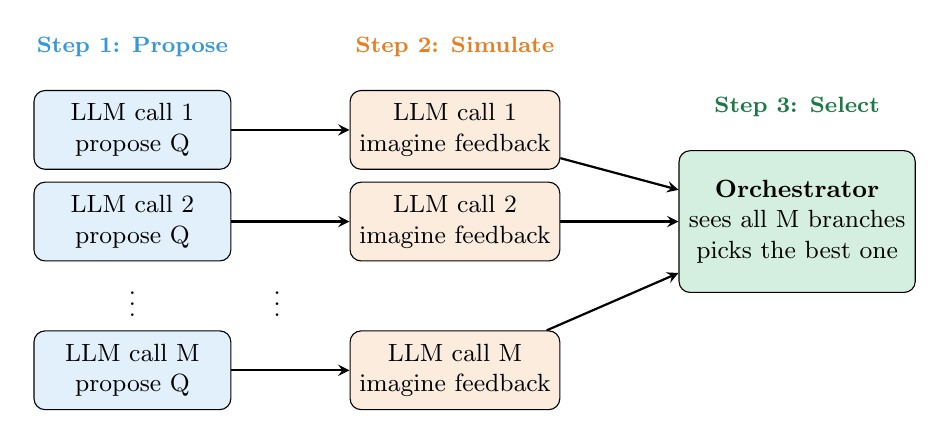
\begin{tikzpicture}[
    node distance=0.6cm and 1.2cm,
    block/.style={rectangle, draw, rounded corners, minimum height=1cm,
                  minimum width=2.5cm, align=center, font=\small},
    arr/.style={->, thick, >=stealth},
  ]
    % Step 1
    \node[block, fill=niceblue!15] (p1) {LLM call 1\\propose Q};
    \node[block, fill=niceblue!15, below=0.15cm of p1] (p2) {LLM call 2\\propose Q};
    \node[below=0.05cm of p2, font=\small] (dots1) {$\vdots$};
    \node[block, fill=niceblue!15, below=0.05cm of dots1] (pm) {LLM call M\\propose Q};

    % Step 2
    \node[block, fill=warningorange!15, right=1.5cm of p1] (s1) {LLM call 1\\imagine feedback};
    \node[block, fill=warningorange!15, right=1.5cm of p2] (s2) {LLM call 2\\imagine feedback};
    \node[right=1.5cm of dots1, font=\small] (dots2) {$\vdots$};
    \node[block, fill=warningorange!15, right=1.5cm of pm] (sm) {LLM call M\\imagine feedback};

    % Step 3
    \node[block, fill=winnergreen!20, right=1.5cm of s2, minimum height=1.8cm,
          minimum width=3cm] (orch) {\textbf{Orchestrator}\\sees all M branches\\picks the best one};

    % Arrows
    \draw[arr] (p1) -- (s1);
    \draw[arr] (p2) -- (s2);
    \draw[arr] (pm) -- (sm);
    \draw[arr] (s1) -- (orch);
    \draw[arr] (s2) -- (orch);
    \draw[arr] (sm) -- (orch);

    % Labels
    \node[above=0.3cm of p1, font=\footnotesize\bfseries, niceblue] {Step 1: Propose};
    \node[above=0.3cm of s1, font=\footnotesize\bfseries, warningorange] {Step 2: Simulate};
    \node[above=0.3cm of orch, font=\footnotesize\bfseries, winnergreen!70!black] {Step 3: Select};
  \end{tikzpicture}
  \end{center}

  \vspace{0.2cm}

  \textbf{Cost:} $2M{+}1$ LLM calls per turn. \quad
  \textbf{LLM decides everything} — no algorithmic scoring.

  \vspace{0.1cm}

  \small
  Works for both DC (suspects/questions) and GN (guesses/feedback).
\end{frame}

%==============================================================================
\section{Guessing Numbers (GN)}
%==============================================================================

\begin{frame}{GN Baseline: LLM Cannot Play Bulls \& Cows}

  \begin{columns}[T]
    \begin{column}{0.48\textwidth}
      \textbf{GN Baseline — 0\% accuracy}

      \begin{table}
        \centering
        \small
        \begin{tabular}{lc}
          \toprule
          \textbf{Metric} & \textbf{Value} \\
          \midrule
          Accuracy & \textcolor{errorred}{\textbf{0\%}} \\
          Avg turns & 25.0 (max) \\
          Tokens & 632K \\
          \bottomrule
        \end{tabular}
      \end{table}

      \vspace{0.2cm}

      \textbf{Example (Puzzle 0, secret = 8362):}

      \small
      \begin{tabular}{ll}
        T14: & Guess 8367 — \textbf{3 bulls!} \\
        T15: & Guess 2591 — 0 bulls \\
        T16: & Guess 9183 — 0 bulls \\
        & \textit{(throws away T14 info)} \\
        T24: & Final: 7359 — wrong \\
      \end{tabular}
    \end{column}

    \begin{column}{0.48\textwidth}
      \begin{alertblock}{Diagnosis}
        The LLM \textbf{ignores feedback}.

        \begin{itemize}
          \item Gets 3/4 digits right at T14
          \item Immediately guesses unrelated numbers
          \item Never returns to the near-miss
          \item Cannot track constraints across turns
        \end{itemize}
      \end{alertblock}

      \vspace{0.2cm}

      \begin{block}{Information-theoretic baseline}
        Optimal play solves Bulls \& Cows in \textbf{5--6 guesses}.

        5040 valid numbers $\xrightarrow{\text{entropy-optimal}}$ 1 in $\sim$5.5 turns.

        LLM can't do this — it doesn't reason about elimination.
      \end{block}
    \end{column}
  \end{columns}
\end{frame}

\begin{frame}{GN + DQS: Results Pending}

  \begin{columns}[T]
    \begin{column}{0.48\textwidth}
      \textbf{What DQS does for GN:}

      \begin{enumerate}
        \item M parallel LLM calls: each proposes a guess
        \item M parallel LLM calls: each imagines the feedback
        \item 1 orchestrator call: picks the most informative guess
      \end{enumerate}

      \vspace{0.3cm}

      \textbf{Key question:}

      Can the LLM select better guesses when it
      \textit{deliberates} about possible outcomes,
      even though it can't track constraints?
    \end{column}

    \begin{column}{0.48\textwidth}
      \begin{table}
        \centering
        \small
        \begin{tabular}{lcc}
          \toprule
          \textbf{Method} & \textbf{Acc} & \textbf{Turns} \\
          \midrule
          GN Baseline & 0\% & 25.0 \\
          GN + DQS & \textit{running} & \textit{running} \\
          \midrule
          \textit{(Optimal)} & \textit{100\%} & \textit{5.5} \\
          \bottomrule
        \end{tabular}
      \end{table}

      \vspace{0.3cm}

      \begin{block}{Expectation}
        DQS may improve over 0\% — but unlikely to match
        optimal play. The LLM's constraint-tracking
        limitation is fundamental.
      \end{block}
    \end{column}
  \end{columns}
\end{frame}

%==============================================================================
\section{Key Findings}
%==============================================================================

\begin{frame}{Week 5 Findings}

  \begin{enumerate}
    \item \textbf{DC: CIP-Lite at Turn 1 is near-optimal for Qwen 7B}

    \small
    Model's case-background comprehension is its best signal.
    NPC responses degrade accuracy monotonically.

    \normalsize
    \vspace{0.3cm}

    \item \textbf{``Improvements'' consistently hurt}

    \small
    AllSuspects: $-$30pp. \quad Ensemble: $-$20pp at 8$\times$ cost.
    7:1 degradation ratio. Consensus anti-correlated with correctness.

    \normalsize
    \vspace{0.3cm}

    \item \textbf{GN: LLM fundamentally cannot track constraints}

    \small
    0\% accuracy on Bulls \& Cows. Ignores feedback, guesses randomly.
    DQS may help question selection but can't fix reasoning.

    \normalsize
    \vspace{0.3cm}

    \item \textbf{The bottleneck is model capability, not the framework}

    \small
    Stopping rules, ensembles, AllSuspects are sound in principle.
    They need a model that can synthesize multi-turn evidence.
  \end{enumerate}
\end{frame}

\begin{frame}{Next Steps}
  \begin{itemize}
    \item \textbf{DQS results} — GN and DC runs in progress
    \item \textbf{Stronger model} — test GPT-4 / Claude to see if
          AllSuspects / Ensemble / DQS become beneficial
    \item \textbf{GN: structured prompting} — step-by-step elimination
          strategy in system prompt (from AR-Bench templates)
    \item \textbf{Larger DC evaluation} — 50+ puzzles for reliable metrics
  \end{itemize}

  \vspace{0.5cm}

  \begin{center}
    \large\textbf{End}
  \end{center}
\end{frame}

\end{document}
